\chapter{Programátorská dokumentace}
V této kapitole popíšeme naší implementaci platformy MHUrho a ukázkové hry. K implementaci platformy bylo použito Visual Studio 2017 Education a .NET Framework 4.7.2, který je zároveň cílovým frameworkem naší platformy. Celá implementace je obsažena v jediném \textit{solution}, MHUrho. 

\section{Struktura solution}

\begin{figure}[h]
	\centering
	\fontsize{10pt}{11pt}\selectfont
	\def\svgwidth{0.9\textwidth}
	\input{img/Project_structure.pdf_tex}
	\caption{Struktura solution. Zelené značí součásti naší práce, oranžové místo budoucí rozšiřitelnosti.}
	\label{fig:solution_structure}
\end{figure}

Hlavním cílem naší práce byla tvorba platformy pro tvorbu RTS her. Jak můžeme vidět v diagramu \ref{fig:solution_structure}, vlastní implementace platformy je realizována několika projekty. Účelem tohoto rozdělení je separace přenositelně implementovatelných částí platformy, které díky využití enginu UrhoSharp a celkovému návrhu práce tvoří velkou většinu funkcionality, od částí závislých na cílovém systému. 

Přenositelné části jsou obsaženy v projektu \texttt{MHUrho}. Výstupem tohoto projektu je knihovna využívaná jak implementacemi pro specifické systémy, tak balíčky tvořícími jednotlivé hry. 

Implementace pro specifické systémy obsahují především inicializační kód, který dostává spuštěný program do konzistentního stavu bez ohledu na platformu, a dále implementace rozhraní specifikovaných v přenositelné části, které umožňují této části pracovat s oblastmi, pro které ani platforma .NET ani používaný herní engine neposkytují přenositelnou implementaci. Tyto oblasti byli popsány v části \ref{sec:system_dif}.

Dále diagram ukazuje dvě součásti solution, které nejsou přímou součástí funkcionality platformy. První z těchto součástí je projekt \texttt{ShowcasePackage}, který obsahuje implementaci ukázkové hry sloužící pro demonstraci schopností platformy a jako referenční implementace pro tvůrce budoucích balíčku. Druhou součástí je \texttt{Installer}, jehož výstupem je \texttt{.msi} instalátor umožňující jednoduchou instalaci platformy na systém Windows spolu s instalací všech závislostí a vložení \textit{Ukázkového balíčku} do nainstalované instance platformy.

\section{Spuštění aplikace}
\label{sec:init}
Spuštění aplikace je specifické pro každý ze systémů. Vzhledem k tomu, že cílem naší práce byla implementace platformy pro systém Windows, popíšeme v této části spuštění aplikace v rámci tohoto systému.

\subsection{Systémová část}

\begin{figure}[h]
	\centering
	\fontsize{8pt}{11pt}\selectfont
	\def\svgwidth{\textwidth}
	\input{img/MHUrhoApp2.pdf_tex}
	\caption{Spouštění aplikace.}
	\label{fig:startup}
\end{figure}

Spuštění začíná v implementaci specifické pro daný systém. Hlavní třídy účastnící se spuštění aplikace a posloupnost volání metod můžeme vidět na obrázku \ref{fig:startup}. U každé ze tříd jsou ilustrovány pouze prvky účastnící se inicializace. 

Pro systém Windows začíná celý proces zavoláním metody \texttt{Program.Main}. Tato metoda jako první inicializuje \texttt{FileManager}, implementující práci se soubory na systému Windows, a uloží ho do statické položky třídy \texttt{MHUrhoApp}. Tento systém je nezbytné inicializovat před spuštěním herního enginu, protože je používán při inicializaci třídy \texttt{MHUrhoApp}.

Jak ukazuje diagram, třída \texttt{MHUrhoApp} je potomkem třídy \texttt{Application} z enginu UrhoSharp. Tato třída, již podle názvu, reprezentuje celou aplikaci v enginu UrhoSharp a poskytuje přístup ke všem součástem enginu. 

Dalším krokem v metodě \texttt{Main} je zpracování parametrů aplikace z příkazového řádku do platformou definované systémově nezávislé reprezentace. Instance třídy \texttt{StartupOptions} obsahující tuto reprezentaci je následně také uložena do statické položky třídy \texttt{MHUrhoApp}, protože je stejně jako \texttt{FileManager} používána při inicializaci MHUrhoApp.

Položky \texttt{FileManager} a \texttt{StartupArgs} jsou statické pro budoucí rozšiřitelnost na platformu Android.
Důvodem je nutnost spuštění enginu pomocí následujícího kódu:

\lstset{
	language=[Sharp]C,
	stringstyle=\color{redstrings}\ttfamily, 
	keywordstyle=\color{bluekeywords},
	morekeywords={ await, new, async}
	emph={MHUrhoApp, ApplicationOptions},
	emphstyle=\color{classgreen}
}
\begin{lstlisting}[]
await surface.Show<MHUrhoApp>(new ApplicationOptions("Data"));
\end{lstlisting}

Metoda \texttt{Show} bohužel nedovoluje přidat konstruktoru \texttt{MHUrhoApp} další parametry, kterými by bylo možné předat \texttt{FileManager} a \texttt{StartupOptions}.

Na systému Windows následuje vytvoření instance \texttt{MHUrhoApp} a zavolání metody \texttt{Run}. Tímto voláním je předána kontrola nad procesem enginu UrhoSharp, který je tímto inicializován a je v něm spuštěna herní smyčka.

V rámci své inicializace zavolá třída \texttt{Application}, reprezentující herní engine, virtuální metodu \texttt{Start}, jejíž přetížením nám umožňuje inicializovat naší část aplikace. Tímto se dostáváme do přenositelné části inicializace.

\subsection{Přenositelná část}

Jak je řečeno v předchozí části, přenositelná část inicializace začíná v okamžiku volání metody \texttt{Start} herním enginem.

V rámci této metody provede naše platforma inicializaci všech svých součástí a přejde do režimu reagování na interakce uživatele s grafickým rozhraním.

Důležitým předpokladem naší platformy i enginu UrhoSharp je přítomnost pouze jedné instance třídy \texttt{MHUrhoApp}, respektive jejího předka \texttt{Application} v dané \texttt{AppDomain}. Vzhledem k tomuto předpokladu je tato jediná instance třídy zpřístupněna pomocí statické proměnné \texttt{Instance}.

Dalšími kroky inicializace jsou:

\begin{enumerate}
	\item Vytvoření \texttt{SynchronizationContextu}, který umožňuje implementaci načítání popsaného v částech \ref{sec:packageloading} a \ref{sec:loading}.
	\item Načtení a nastavení konfigurace aplikace za využití třídy \texttt{FileManager} inicializované v systémové části. Toto nastavení ovlivňuje například vzhled okna aplikace či vykreslovanou vzdálenost ve hře.
	\item Načtení seznamu přítomných balíčků, popsané blíže v části \ref{fig:packagemanager}. Při chybě v načítání kteréhokoli z balíčků je po spuštění uživatelského rozhraní uživateli zobrazeno hlášení o této chybě.
	\item Inicializace vstupu a výstupu. Tato inicializace je implementována podle návrhového vzoru \textit{Factory} pro zjednodušení přepínání mezi různými schématy vstupu a výstupu. V rámci naší práce je implementováno pouze schéma myši a klávesnice, ale v implementaci platformy je připravena základní struktura pro implementaci schématu pro dotykové obrazovky. 
\end{enumerate}

Tímto je inicializace kompletní. Volání metody \texttt{Start} se vrací do metody \texttt{Run}, ve které engine předchází do smyčky obsluhující události uživatelského vstupu.

\section{Uživatelské rozhraní}

\begin{figure}[h]
	\centering
	\fontsize{8pt}{11pt}\selectfont
	\def\svgwidth{\textwidth}
	\input{img/UIReferences.pdf_tex}
	\caption{Datová struktura uživatelského rozhraní.}
	\label{fig:uireferences}
\end{figure}

Jak můžeme vidět na diagramu \ref{fig:uireferences}, centrálními třídami uživatelského rozhraní v rámci menu jsou třídy \texttt{MenuController} a \texttt{MenuUIManager}. Dále můžeme vidět, že z pohledu herního enginu je grafické rozhraní reprezentováno třídou \texttt{UI} s kořenovým prvkem \texttt{Root}.

Účelem třídy \texttt{MenuController} je odstínění implementace uživatelského rozhraní od detailů implementace zbytku platformy. Pokud je tedy výsledkem uživatelovi akce změna stavu jiné části platformy než UI, je tato akce delegována právě třídě \texttt{MenuController}. Zároveň se také tato třída snaží odstiňovat zbytek platformy od implementace uživatelského rozhraní, tedy pokud část hry požaduje změnu uživatelského rozhraní, měla by tuto akci delegovat třídě \texttt{MenuController}.

Třída \texttt{MenuUIManager} je, jak můžeme vidět, centrálním bodem implementace uživatelského rozhraní menu. Její hlavní funkcí je management obrazovek menu, implementace přepínání mezi nimi a poskytnutí přístupu k třídám reprezentujícím tyto obrazovky. V rámci přepínání obrazovek umožňuje tato třída jednoduše přepínat zpět na předchozí obrazovky, protože při každém přepnutí na novou obrazovku je stará obrazovka přidána do zásobníku předchozích obrazovek.

Každá z obrazovek menu je reprezentována samostatnou třídou implementující chování obrazovky a zajišťující správu prostředků herního enginu příslušících dané obrazovce. Jak můžeme vidět na diagramu \ref{fig:uireferences}, slouží každá ze tříd reprezentujících obrazovky menu jako \textit{proxy} pro třídu, která implementuje chování obrazovky a je vlastníkem prostředků enginu pro její zobrazení uživateli. 

Z pohledu enginu tvoří uživatelské rozhraní strom s kořenem \texttt{Root}. Každá obrazovka je tedy dítětem tohoto kořenu, s dalšími prvky jako tlačítky a popisky jako svými dětmi. Tyto prostředky, reprezentující danou obrazovku, jsou spravovány právě implementační třídou a mají stejnou životnost jako tato třída.

Zobrazení obrazovky je uskutečněno v reakci na zavolání metody \texttt{Show} na \textit{proxy} třídě obrazovky. Metoda \texttt{Show} vytvoří novou instanci implementační třídy, která v rámci konstruktoru použije engine a \texttt{UI.Root} pro nahrání obrazovky. Při následném skrytí obrazovky v reakci na volání metody \texttt{Hide} na proxy třídě je implementační třída zahozena pomocí volání \texttt{Dispose} a nastavení reference na null. V rámci volání \texttt{Dispose} jsou z reprezentace uživatelského rozhraní uvnitř enginu odstraněny všechny prvky příslušící této obrazovce. Díky této implementaci nedochází k hromadění naalokovaných obrazovek i při cyklickém přepínání mezi několika obrazovkami.



\subsection{Definice vzhledu}
Engine UrhoSharp umožňuje definici rozložení a vzhledu uživatelského rozhraní jak v kódu, tak pomocí XML souborů. Podle složitosti jednotlivých obrazovek používáme kombinaci obou těchto možností. Některé jednodušší obrazovky, jako například hlavní menu, mají celý svůj vzhled definován pomocí XML souborů. Složitější obrazovky, měnící svůj vzhled v reakci na uživatelské akce, mají základní vzhled definován pomocí XML a následně měněn pomocí kódu dané obrazovky. 

\noindent{Použité XML soubory se rozdělují na dva druhy:}
\begin{enumerate}
	\item definující vzhled,
	\item definující rozložení.
\end{enumerate}

Soubory definující uživatelské rozhraní platformy pro systém Windows jsou uloženy v adresáři \texttt{MHUrho.Desktop/Data/UI/}.
Vzhled prvků rozhraní je definován především v souboru \texttt{MainMenuStyle.xml}, spolu s několika menšími soubory pojmenovanými \uv{\texttt{...Style.xml}}, definujícími vzhled dynamicky přidávaných prvků. Hlavní styl uživatelského rozhraní \texttt{MainMenuStyle.xml} je nastaven v kořeni \texttt{UI.Root} jako \textit{defaultní}, je tedy aplikován na všechny prvky v celém stromu, pokud jim není explicitně přiřazen jiný vzhled.

Rozložení prvků je pro každou obrazovku definováno v separátním souboru, pojmenovaném \texttt{[Jméno obrazovky]Layout.xml}. Tyto soubory byli vytvořeny za použití editoru enginu Urho3D, který je distribuován spolu s enginem UrhoSharp. 

\subsection{Přepínání obrazovek}
Přepínání obrazovek je jedním z hlavních úkolů třídy \texttt{MenuUIManager}. Tato třída poskytuje metody pro přepnutí na každou z obrazovek menu, spolu s uložením aktuální obrazovky na zásobník předchozích obrazovek pro možnost návratu. Každá z  metod pro přepnutí obrazovek deklaruje data potřebná pro zobrazení nové obrazovky, která následně poskytne třídě reprezentující danou obrazovku.

Posloupnost možných přechodů obrazovek můžeme vidět na diagramu \ref{fig:screen_structure}. Při spuštění aplikace je počáteční obrazovkou hlavní menu. Jak můžeme vidět na diagramu, z tohoto menu se lze dostat na obrazovky \textit{Package picking}, \textit{Load game}, \textit{Options} a \textit{About}. Dále lze z tohoto menu ukončit celou aplikaci. Každý z černých přechodů přidává starou obrazovku na zásobník obrazovek a nastavuje novou obrazovku jako \texttt{CurrentScreen}, tedy aktuální obrazovku. Tímto způsobem poskytuje třída \texttt{MenuUIManager} implementaci tlačítka zpět, které je schopno vracet se v protisměru černých šipek.

Červené šipky v diagramu značí přechod do hry, který vyčistí zásobník obrazovek a zahodí aktuální obrazovku. Tímto je uvolněna veškerá nepotřebná paměť zabraná uživatelským rozhraním menu a je přenechána pro běh hry.

Dále můžeme vidět přerušované šipky, které značí přechody bez možnosti návratu touto cestou. Při pozastavení úrovně je hra převedena do obrazovky \textit{Pauza}. Tato obrazovka se mírně liší podle toho, zda jsme se do ní dostali dostali z editované či hrané úrovně. Tento rozdíl je implementován podle návrhového vzoru Strategy.

\begin{figure}[h]
	\centering
	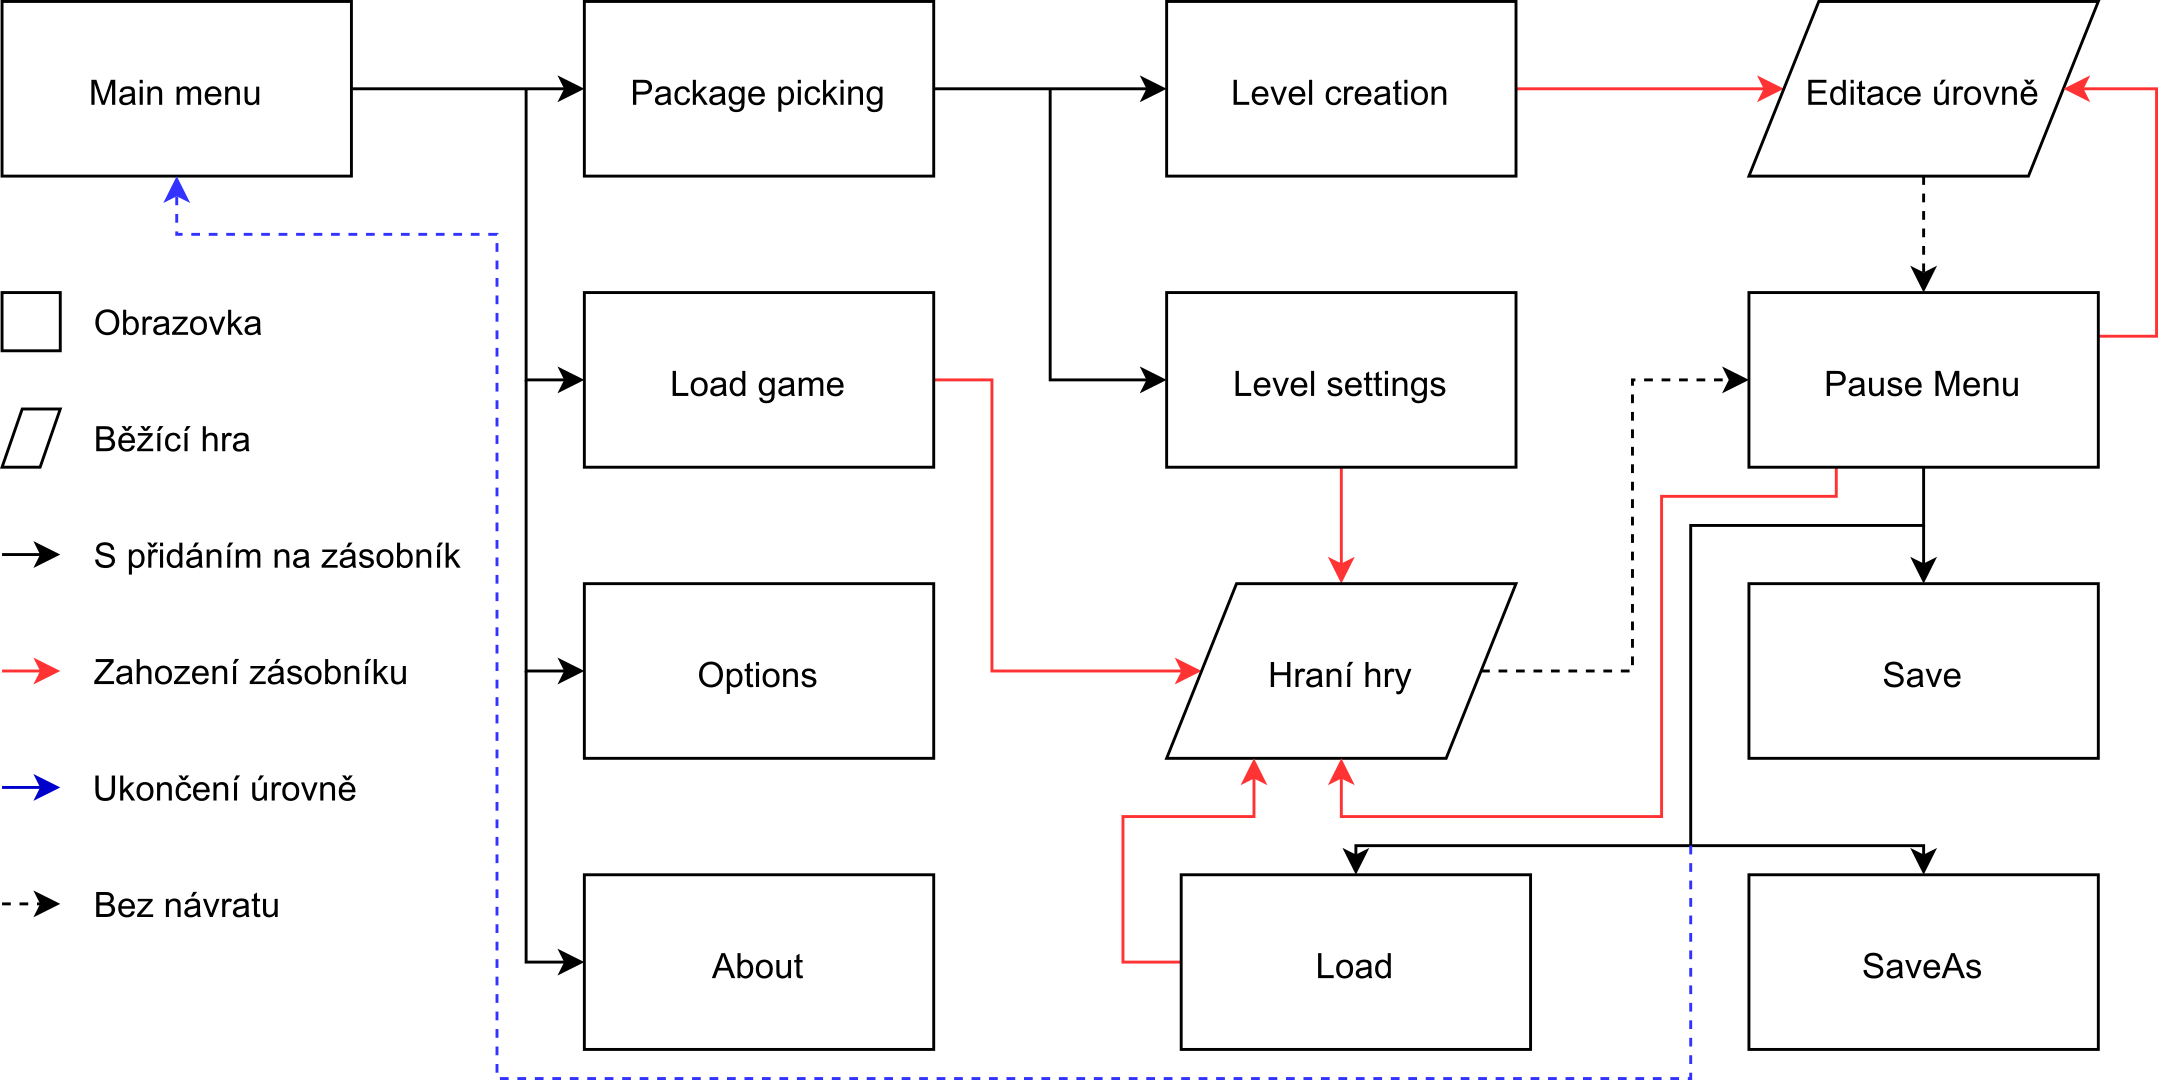
\includegraphics[width=\textwidth]{img/ScreenStructure.png}
	\caption{Obrazovky menu a přechody mezi nimi.}
	\label{fig:screen_structure}
\end{figure}


Vlastní akce přepnutí obrazovky je implementována vytvořením instance implementační třídy, která v rámci svého konstruktoru vytvoří danou obrazovku. Toto vytvoření probíhá za použití souborů definujících rozložení prvků, které jsou voláním \texttt{UI.LoadLayoutToElement} použity pro vytvoření objektové reprezentace uživatelského rozhraní uvnitř enginu. Tato objektová reprezentace je následně přístupná i z našeho kódu, a je použitá pro další modifikace, například v reakci na akci uživatele.

Herní data potřebná pro zobrazení některých obrazovek, například herní balíček při zobrazení výběru úrovní, jsou zpřístupněna jako veřejná \textit{property} proxy tříd. Při zavolání metody \texttt{Show} je kontrolována přítomnost a validita poskytnutých dat. Implementační třída při své alokaci dostává referenci na proxy třídu, čímž jí je umožněn přístup k poskytnutým herním datům a je schopna tato data použít pro zobrazení obrazovky.

\subsection{Automatizace uživatelského rozhraní}

Pro účely testování byl vytvořen systém pro automatické přepínání obrazovek bez zásahu uživatele. Tento systém je možné použít vytvořením XML souboru a specifikací parametrů příkazové řádky.

Parametrem spouštějícím tento systém je \uv{-ui [d|s] xmlFilePath}, který z kombinace poskytnuté cesty a přepínačů \uv{d|s} vytvoří cestu, z které nahraje XML soubor. Přepínače \uv{d|s} určují, zda je cesta \uv{xmlFilePath} relativní vůči adresáři aplikace či adresáři dynamických dat, blíže popsaném v části \ref{sec:packagedir}. Soubor XML musí být validní vůči schématu \texttt{MenuActions.xsd}. Z tohoto souboru jsou  nahrány třídy specifikující akce pro jednotlivé obrazovky. Tyto třídy jsou potomkem \texttt{MenuScreenAction} a jsou vždy určeny pro konkrétní obrazovku. Implementace každé z obrazovek zná sobě příslušící třídu a umí v ní zakódovanou akci vykonat. Dále je vytvořena instance \texttt{ActionManager}, která slouží jako úložiště těchto nahraných tříd a řídí jejich předávání jednotlivým obrazovkám.

Diagram \ref{fig:uiautomationload} je zjednodušením diagramu \ref{fig:startup} a ukazuje části inicializace platformy, ve kterých je prováděn tento systém. Jak můžeme vidět, při startu aplikace bez parametrů příkazové řádky je tento systém úplně přeskočen. 

\begin{figure}[h]
	\centering
	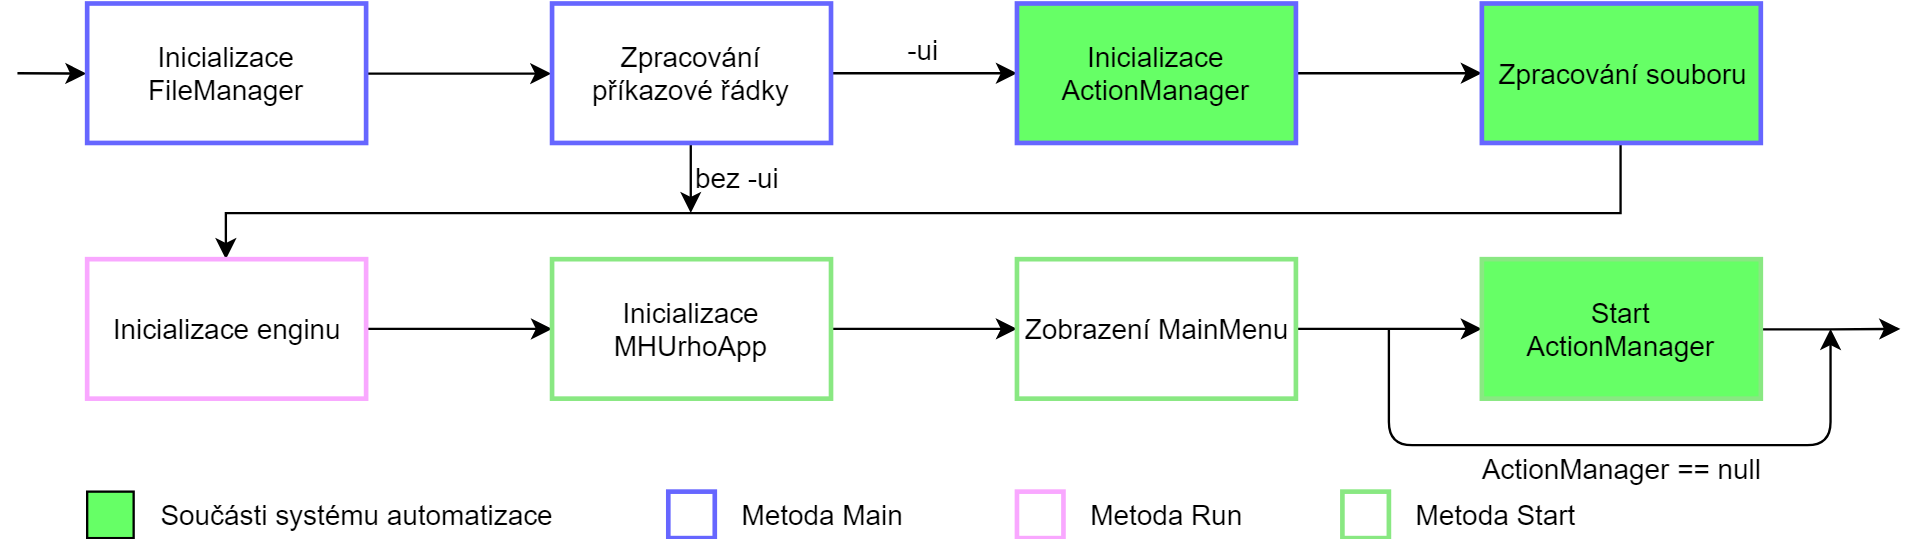
\includegraphics[width=\textwidth]{img/MenuActions.png}
	\caption{Nahrávání akcí v průběhu inicializace platformy.}
	\label{fig:uiautomationload}
\end{figure}

\section{Systém balíčků}
V části \ref{sec:packagestructure} jsme popsali základní strukturu systému balíčků, jejich popis pomocí XML souboru a podporované formáty dat pro nahrávání do hry. V této části popíšeme implementaci této funkcionality.

\subsection{Adresář balíčků}
\label{sec:packagedir}
Při instalaci hry je vytvořen adresář, ve kterém jsou uložena data generovaná aplikací či přidávaná uživatelem do aplikace. Tento adresář je v kódu označován jako \texttt{DynDataDir}, tedy adresář pro dynamická (měnící se) data. Jako součást tohoto adresáře je při instalaci vytvořen podadresář \texttt{Packages}, jehož účelem je centralizované umístění balíčků.

Obsah tohoto podadresáře můžeme vidět na diagramu \ref{fig:packagesdir}. Z pohledu platformy nejdůležitějším obsahem je soubor \texttt{Packages.xml}, ve kterém jsou uloženy záznamy o všech balíčcích dostupných ve hře. Tento soubor je ve formátu XML, splňujícím schéma \texttt{MHUrho.Desktop/Data/Schemas/GamePack.xsd}. Záznamy je možné do tohoto souboru přidávat dvěma způsoby. Prvním je pomocí grafického rozhraní při běhu platformy, konkrétně stisknutím tlačítka \texttt{Add} na obrazovce pro výběr balíčků \texttt{PackagePickingScreen}. Druhým je manuální editace soubor \texttt{Packages.xml}, při které musí být dodrženo schéma souboru. Tímto způsobem je tedy možné přidat balíčky mimo běh platformy. 

\begin{figure}[h]
	\centering
	\fontsize{6pt}{7pt}\selectfont
	\def\svgwidth{0.7\textwidth}
	\input{img/DynData.pdf_tex}
	\caption{Typická struktura adresáře \texttt{DynDataDir}.}
	\label{fig:packagesdir}
\end{figure}

Tato struktura ukládání balíčků je vystavěna s myšlenkou uložení všech balíčků jako podadresářů adresáře \texttt{Packages}. Tato vlastnost ale není nijak vynucována či kontrolována, je tedy možné přidat i balíčky mimo tento adresář. Jedinou překážkou je nutnost použití relativní cesty vůči adresáři \texttt{Packages}.

\subsection{PackageManager}
\label{sec:packagemanager}
Třída \texttt{PackageManager} je základem celého systému balíčků. Jak můžeme vidět v části \ref{sec:init} na obrázku \ref{fig:startup}, vytvoření instance \texttt{PackageManager} je součástí inicializace platformy. První akcí na takto vytvořené instanci je načtení souboru \texttt{Packages.xml}, popsaného v předchozí části \ref{sec:packagedir}.

\begin{figure}[h]
	\centering
	\fontsize{8pt}{11pt}\selectfont
	\def\svgwidth{\textwidth}
	\input{img/PackageManager.pdf_tex}
	\caption{Datová struktura balíčků.}
	\label{fig:packagemanager}
\end{figure}

Na diagramu \ref{fig:packagemanager} můžeme vidět datovou strukturu systému balíčků. Při načtení souboru \texttt{Packages.xml}, případně při přidání balíčku do běžící hry, je pro každý balíček vytvořena jedna instance třídy \texttt{GamePackRep}, která je použita pro prezentaci tohoto balíčku uživateli při výběru pro načtení na obrazovce \texttt{PackagePickingScreen}. Instance třídy \texttt{GamePackRep} obsahuje pouze data potřebná pro její použití, tedy pro prezentaci balíčku a případné následné načtení balíčku. Těmito daty jsou:

\begin{itemize}
	\item jméno,
	\item popis,
	\item ikona,
	\item cesta k XML souboru.
\end{itemize}

Tato data jsou z XML souboru balíčku načtena při startu hry či přidání balíčku a zůstávají přítomna v paměti až do ukončení hry. Zbylá data balíčku jsou načítána až po zvolení jednoho konkrétního balíčku hráčem. Ve hře je vždy nejvýše jeden načtený balíček, dostupný jako \texttt{ActivePackage} na třídě \texttt{PackageManager}.

Druhou funkcí třídy \texttt{PackageManager} je obalení rozhraní třídy \texttt{ResourceCache} poskytované enginem UrhoSharp. Tato třída umožňuje načítaní všech druhů assetů podporovaných enginem a jejich cachování. Bohužel přístup k této třídě je omezen na hlavní vlákno aplikace, tedy při přístupu z jiného vlákna, ve kterém implementujeme načítání hry, dochází k pádu aplikace. Pro zamezení chyb při programování načítání jsme vytvořili identické rozhraní na třídě \texttt{PackageManager}, které automaticky přesměrovává všechna volání na hlavní vlákno aplikace, kde následně zavolá odpovídající metodu \texttt{ResourceCache}.


\subsection{GamePack}
\label{sec:gamepack}


Třída \texttt{GamePack} představuje kompletně načtený balíček. Jak můžeme vidět na diagramu \ref{fig:packagemanager}, obsahuje tato třída referenci na instanci \texttt{GamePackRep} reprezentující daný balíček. Dále obsahuje tyto data:

\begin{itemize}
	\item typy dlaždic,
	\item typy jednotek,
	\item typy budov,
	\item typy projektilů,
	\item typy surovin,
	\item typy hráčů,
	\item typy logik úrovní,
	\item seznam úrovní,
	\item defaultní typ dlaždice,
	\item textury ikon.
\end{itemize}

Tato data jsou načítána podle jejich popisu v XML souboru, splňujícího schéma \texttt{MHUrho.Desktop/Data/Schemas/GamePack.xsd}. Soubor je vůči tomuto schématu validován jak při načítání reprezentanta balíčku (\texttt{GamePackRep}), tak při načítání celého balíčku. Pro zjednodušení manipulace s tímto XML souborem v naší platformě jsme vytvořili třídy v souboru \texttt{GamePackXml.cs}, které tvoří objektovou reprezentaci tohoto schématu. Pokud je tedy v elementu \texttt{TileType} požadován potomek \texttt{texturePath}, pak \textit{singleton} instance třídy \texttt{TileTypeXml} bude obsahovat položku \texttt{TexturePath}, kterou bude možno použít v metodě \texttt{XElement.Element()} jako argument pro získání tohoto potomka. Tímto způsobem je izolován zbytek kódu platformy od změn ve formátu či jménech elementů ve schématu. Další výhodou tohoto přístupu, a důvodem použití návrhového vzoru \textit{Singleton}, je reprezentace dědičnosti ve schématu pomocí dědičnosti v jeho objektové reprezentaci.

Při hře slouží třída \texttt{GamePack} jako databáze typů, tedy obsahuje metody pro získání reference na typy z výčtu výše podle jména či podle číselného identifikátoru. Jméno i identifikátor jsou načítány z XML souboru, ve kterém je jejich přítomnost vyžadována schématem. Systém typů je blíže popsán v části \ref{sec:types}.

Poslední funkcí je přístup k úrovním obsaženým v balíčku. Úrovně jsou, podobně jako balíčky samotné, před vlastním načtením reprezentovány separátní třídou \texttt{LevelRep}. Tato třída, podobně jako \texttt{GamePackRep}, obsahuje data potřebná pro výběr a nastavení úrovně před jejím spuštěním. Dále tato třída umožňuje manipulaci s úrovní z pohledu assetu, tedy její ukládání při editaci, vytvoření kopie pro editaci, načtení pro hru atd. Toto chování je implementováno podle návrhového vzoru \textit{State}.

\subsection{Assety}
\label{sec:assets}
Pojmem assety označujeme v naší práci veškerá data použitelná pro implementaci hry. Patří mezi ně například:

\begin{itemize}
	\item 3D modely,
	\item textury,
	\item XML data,
	\item části logiky poskytované enginem.
\end{itemize}

Každý typ entity, tedy budovy, jednotky či projektilu, má definovanou svou množinu assetů, které ji reprezentují při zobrazení či při výpočtu kolizí. Pro dodání assetů instancím těchto typů poskytujeme tři způsoby definice.

Prvním způsobem je explicitní specifikace assetů přímo v XML souboru balíčku. Tento způsob je implementován třídou \texttt{ItemsAssetContainer}, která z XML elementu vyčte všechna potřebná data a při požadavku vytvoří reprezentaci entity v herním enginu. Bližší popis reprezentace hry v herním enginu můžete nalézt v části \ref{sec:engineview}.

Druhým způsobem je využití funkcionality poskytované herním enginem a s ním distribuovaným editorem. V tomto editoru lze definovat reprezentaci entity a následně tuto definici serializovat do XML či binárního souboru, do takzvaného \textit{prefab}, neboli prefabrikátu. Pro tento způsob poskytujeme dvě třídy, \texttt{XmlPrefabAssetContainer} a \texttt{BinaryPrefabAssetContainer}, které obalí soubor definující reprezentaci entity a při žádosti o vytvoření instance entity použijí engine a tyto soubory pro její vytvoření.

Použitý způsob vytváření je specifikován v XML popisu typu entity, a v závislosti na zvoleném způsobu jsou dále požadována další data, specifická pro daný způsob. Použití XML či Binary prefab umožňuje využití všech možností UrhoSharp enginu. Námi implementovaný \texttt{ItemsAssetContainer} umožňuje zjednodušenou specifikaci bez externích nástrojů, jakým je editor Urho3D, zato ale omezuje použitelné součásti enginu na tuto podmnožinu:

\begin{itemize}
	\item \texttt{Static model},
	\item \texttt{Animated model},
	\item \texttt{Collision shape},
	\item nastavení \texttt{Scale}.
\end{itemize}

Ke každému z modelů navíc umožňuje definovat jeho textury. Tato podmnožina je podle nás dostatečná pro tvorbu graficky jednodušších her,

\subsection{Načítání balíčku}
\label{sec:packageloading}

Načítání balíčku je implementováno metodou \texttt{Load}, jejíž prototyp je:
\begin{lstlisting}
public static async Task<GamePack> Load(string pathToXml,
GamePackRep gamePackRep,
XmlSchemaSet schemas,
IProgressEventWatcher loadingProgress = null)
\end{lstlisting}

Už podle deklarace metody vidíme, že se implementace pokouší o asynchronní načítání balíčku. Nejedná se o úplné asynchronní načítání v pravém slova smyslu, protože drtivou většinu dat je nutno načítat na hlavním vlákně z důvodu restrikcí herního enginu, blíže popsaným v části \ref{sec:packagemanager}. Hlavním cílem je tedy rozdělit načítání na části, mezi kterými je platforma schopna nadále zpracovávat vstup od hráče. Tímto se snažíme zamezit tzv. \uv{zamrzání} aplikace, kdy aplikace z pohledu uživatele nic nedělá a odmítá reagovat na jakýkoli vstup od hráče. V prvních verzích bez tohoto přístupu jsme naráželi na problém, kdy systém Windows považoval náš proces za mrtvý a navrhoval nám jej zabít. Touto implementací jsme tomuto problému zabránili a navíc jsme umožnili notifikovat hráče o průběhu načítání.

Z pohledu implementace vlastního načítání je princip vcelku jednoduchý. Posloupnost akcí je následovná:

\begin{enumerate}
	\item načíst a validovat XML soubor;
	\item načíst typy dlaždic, jednotek, budov, projektilů, surovin;
	\item načíst typy logik hráčů a úrovní;
	\item načíst textury ikon;
	\item načíst reprezentanty úrovní,
	\item zavřít XML soubor.
\end{enumerate}

Při jakékoli chybě načítání, ať už nevalidnímu XML či chybějícímu souboru některého assetu, je načítání zastaveno, dosud načtená data znovu odalokována, chyba zalogována a zpět vypuštěna výjimka typu \texttt{PackageLoadingException}, signalizující chybu při načítání balíčku.

\section{Logika hry}
V této sekci popíšeme implementaci vlastního průběhu hry, nejdříve z pohledu herního enginu a následně z pohledu naší platformy. Oba tyto pohledy jsou poskytnuty tvůrcům balíčků pro tvorbu pluginů.

\subsection{Herní engine}
\label{sec:engineview}

\begin{figure}[h]
	\centering
	\fontsize{8pt}{11pt}\selectfont
	\def\svgwidth{\textwidth}
	\input{img/EngineRepre.pdf_tex}
	\caption{Reprezentace hry z pohledu herního enginu.}
	\label{fig:scenegraph}
\end{figure}


Diagram \ref{fig:scenegraph} ukazuje reprezentaci hry z pohledu herního enginu. Aktuálně spuštěná úroveň je v herním enginu reprezentována tzv.~\textit{Scene graph} strukturou, tedy grafem scény. Tento graf je strom s vrcholy typu \texttt{Node}. Kořenem tohoto stromu je instance třídy \texttt{Scene}, která je specializací \texttt{Node}.

Diagram \ref{fig:scenegraph} ukazuje část grafu scény, ve které můžeme vidět jeho základní strukturu. Názvy v instancích třídy \texttt{Node} ukazují, který herní objekt daná instance reprezentuje. Všechny jsou ale instancí stejné třídy \texttt{Node}. Oproti tomu názvy komponentů ukazují jméno třídy, jejíž jsou instancí. Tyto třídy jsou pouze potomkem třídy \texttt{Component}. Tento rozdíl vychází z návrhu enginu, ve kterém je k přidávání uživatelské logiky zamýšlena třída \texttt{Component}. Třída \texttt{Node} obecně není určena pro vytváření potomků.

Na diagramu můžeme vidět stav hry, ve kterém jsou v herním světě umístěny dvě budovy, jednotka a projektil. Vztah \texttt{Component} a \texttt{Node} v naší platformě je blíže popsán v části \ref{sec:platformimpl}. Dále můžeme vidět mapu a její reprezentaci. Tato reprezentace je blíže popsána v části \ref{sec:mapimpl} a \ref{sec:mapimpldoc}. Jak můžeme vidět na diagramu, lze \texttt{Node} použít k reprezentaci jedné entity, částí entit nebo skupiny entit. Příkladem reprezentace částí může být právě rozdělení mapy na \uv{Chunky}. Budovy, jednotky či projektily mohou mít pod touto jednou \texttt{Node} také přidány podstrom, reprezentující jejich součást. Za reprezentaci skupiny entit jednou \texttt{Node} můžeme považovat situaci, kdy kamera sleduje jednotku. V tu chvíli \texttt{Node} dané jednotky reprezentuje jak jednotku samotnou, tak kameru, a obě současně přesouvá v herním světě.



Každá instance třídy \texttt{Node} má několik atributů, které umožňují její umístění v herním světě a další manipulaci. Nejdůležitějšími z těchto atributů jsou:

\begin{itemize}
	\item \texttt{Position} (pozice),
	\item \texttt{Rotation} (rotace),
	\item \texttt{Scale} (velikost),
	\item \texttt{Enabled}.
\end{itemize}

Již podle názvu slouží \texttt{Position} a \texttt{Rotation} pro umístění dané \texttt{Node} do herního světa a určení jejího otočení. Obě tyto vlastnosti jsou počítány vůči rodičovské \texttt{Node}, jak můžeme vidět na obrázku \ref{fig:relativeposition}. Atribut \texttt{Scale} určuje závislost souřadnic v podstromu této \texttt{Node} na souřadnicích vzhledem k souřadnicím v podstromu otce této \texttt{Node}. Na ukázce můžeme vidět dvě \texttt{Node}, kdy levá horní \texttt{Node} je otcem pravé spodní \texttt{Node}. Otec je umístěn na pozici \((1,0,1)\) a má nastaven \texttt{Scale} na \((2,2,2)\). Potomek má vlastní atribut \texttt{Position} nastaven na \((1,0,1)\). Výslednou pozicí potomka v herním světě, označovanou jako \texttt{WorldPosition}, pak získáme tímto výpočtem:\[\scalebox{0.9}{Potomek.WorldPosition = Otec.WorldPosition + Potomek.Position * Předek.Scale}\] Díky tomu bude výsledná pozice potomka v herním světě \((3,0,3)\). Použitá \texttt{WorldPosition} otce je vypočítána stejným způsobem.

\begin{figure}[h]
	\centering
	\fontsize{8pt}{11pt}\selectfont
	\def\svgwidth{\textwidth}
	\input{img/RelativePosition.pdf_tex}
	\caption{Ukázka výpočtu pozice \texttt{Node} v herním světě.}
	\label{fig:relativeposition}
\end{figure}

Pro implementaci chování hry lze na každou instanci třídy \texttt{Node} připojit potomky třídy \texttt{Component}. Hlavním způsobem implementace logiky při použití herního enginu UrhoSharp je vytvoření vlastních specializací třídy \texttt{Component}, implementace virtuálních metod a přidání této naší komponenty k instanci \texttt{Node} v grafu scény. Tímto způsobem je vytvořena také implementace naší platformy, blíže popsána v části \ref{sec:platformimpl}. 

Engine sám poskytuje několik základních typů komponent, implementujících nejčastější potřeby her. Těmito typy jsou:

\begin{itemize}
	\item \texttt{StaticModel} pro vykreslování bez animací,
	\item \texttt{AnimatedModel} pro vykreslování s animacemi,
	\item \texttt{RigidBody} pro simulaci fyziky,
	\item \texttt{CollisionShape} pro výpočet kolizí ve spolupráci s \texttt{RigidBody},
	\item \texttt{Camera} pro vykreslení na obrazovku,
	\item \texttt{Light} pro přidání světla.
\end{itemize}

Jak bylo řečeno v části \ref{sec:assets}, umožňuje platforma tvůrcům balíčků specifikovat assety příslušící jednotlivým typům jednotek mnoha způsoby. Všechny tyto způsoby ale využívají tento popis právě k vytvoření instancí \texttt{Node} a \texttt{Component}, které jsou spojeny a inicializovány podle uložených dat. 

Vlastní výpočet stavu hry je iniciován enginem, který ve všech prvcích grafu scény, tedy \texttt{Node} i \texttt{Component}, zavolá jejich virtuální metodu \texttt{OnUpdate}. Tato metoda je volána s parametrem \texttt{timeStep}, který představuje čas uběhlý od předchozího výpočtu stavu. V rámci této metody provádí standardní i uživatelské komponenty výpočet následujícího stavu.

Zmíněný atribut \texttt{Enabled} třídy \texttt{Node} ovlivňuje šíření volání metody \texttt{OnUpdate}. Pokud je tento atribut nastaven na hodnotu \texttt{false}, není na dané instanci \texttt{Node} ani na jejím podstromu proveden \uv{update}. Tento atribut je přítomný i na třídě \texttt{Component}, na které ovládá volání \texttt{OnUpdate} na dané instanci \texttt{Component}.

\subsection{Pohled platformy}
\label{sec:platformimpl}

\begin{figure}[h]
	\centering
	\fontsize{8pt}{11pt}\selectfont
	\def\svgwidth{\textwidth}
	\input{img/PlatformStructure.pdf_tex}
	\caption{Třída \texttt{LevelManager}.}
	\label{fig:platform}
\end{figure}

Z pohledu platformy se hra skládá z několika částí, ilustrovaných na diagramu \ref{fig:platform}. Vztah některých těchto částí s grafem scény popsaným v části \ref{sec:engineview} můžeme vidět na diagramu \ref{fig:scenegraph}.

Centrální částí je instance třídy \texttt{LevelManager}, která slouží jako přístupový bod ke všem součástem tvořících implementaci platformy. Dále tato třída slouží jako databáze všech budov, jednotek, projektilů a hráčů přítomných ve hře., Pro budovy, jednotky a projektily umožňuje dále jejich vytvoření či zničení. Jak můžeme vidět na diagramu \ref{fig:scenegraph}, je tato třída potomkem třídy \texttt{Component} a je připojena k \texttt{Node} obsahující jako podstrom celý zbytek herního světa. Tímto způsobem je pohled platformy spojen s pohledem herního enginu.

Každá entita, tedy každá budova, jednotka či projektil je reprezentována instancí odpovídající třídy implementující chování tohoto druhu. Těmito třídami jsou \texttt{Building}, \texttt{Unit} a \texttt{Projectile}. Jak můžeme vidět na diagramu \ref{fig:componenthierarchy}, jsou všechny tyto třídy potomkem třídy \texttt{Entity}, která je sama potomkem třídy \texttt{Component}. Tímto způsobem je provázána reprezentace entity z pohledu herního enginu a z pohledu platformy. 


\begin{figure}[h]
	\centering
	\fontsize{9pt}{11pt}\selectfont
	\def\svgwidth{0.7\textwidth}
	\input{img/PlatformHier.pdf_tex}
	\caption{Potomci třídy \texttt{Component} v platformě.}
	\label{fig:componenthierarchy}
\end{figure}

\subsection{Typy}
\label{sec:types}
Platforma zavádí systém typů herních prvků. Tento systém je separován od typového systému jazyka a je aplikován pro tyto prvky:
\begin{itemize}
	\item logiky úrovně (\texttt{LevelLogicType}),
	\item hráče (\texttt{PlayerType}),
	\item dlaždice (\texttt{TileType}),
	\item budovy (\texttt{BuildingType}),
	\item jednotky (\texttt{UnitType}),
	\item projektily (\texttt{ProjectileType}),
	\item suroviny (\texttt{ResourceType}).
\end{itemize}

Pro každý z druhů prvků definuje typ jejich vzhled a/nebo chování. Vzhled je definován pomocí množiny assetů specifikovaných v XML elementu definujícím tento typ, které jsou následně použity při vytváření herních prvků tohoto typu. Chování je definováno pomocí systému pluginů, popsaných v části \ref{sec:plugins}. 

Výjimkou z tohoto pravidla jsou typy surovin, které ve hře nemají vlastní instance a jsou používány pouze jako klíč pro přístup k množství daného typu suroviny vlastněného hráčem.

Každá instance výše vyjmenovaných druhů herních prvků obsahuje referenci na svůj typ. Příklad můžeme vidět na diagramu \ref{fig:pluginstructure}, kde vidíme instance \texttt{Building}, tedy budov, které obsahují reference na instance \texttt{BuildingType} reprezentující typ budov \textit{Gate}, tedy brána, nebo \textit{Wall}, tedy zeď.

Typy jsou jednou z hlavních částí obsahu balíčku. Instance reprezentující jednotlivé typy jsou vytvořeny při načtení balíčku a zanikají při odalokování balíčku. 

\subsection{Pluginy}
\label{sec:plugins}
Hlavním cílem naší práce bylo umožnit tvůrcům balíčků použít jazyk C\# pro tvorbu logiky hry ve formě pluginů. Návrh tohoto systému a použité technologie byl popsán v části \ref{sec:logicandplugins}. Platforma definuje dva druhy pluginů:

\begin{enumerate}
	\item pluginy typů,
	\item pluginy instancí.
\end{enumerate}

Ukázku zapojení těchto pluginů do struktury hry můžeme vidět na diagramech \ref{fig:simplepluginstructure} a \ref{fig:pluginstructure}. Diagram \ref{fig:simplepluginstructure} ukazuje základní princip propojení pluginů, instancí herních prvků a typů těchto herních prvků. Tyto vztahy jsou dále popsány v následující části \ref{sec:typeplugins}. Diagram \ref{fig:pluginstructure} obsahuje ukázku několika budov v herním světě různých typů s jejich pluginy.

\begin{figure}[h]
	\centering
	\fontsize{8pt}{11pt}\selectfont
	\def\svgwidth{\textwidth}
	\input{img/SimplePluginStructure.pdf_tex}
	\caption{Princip zapojení pluginů do struktury hry.}
	\label{fig:simplepluginstructure}
\end{figure}

\subsubsection{Pluginy typů}
\label{sec:typeplugins}
Jak jsme popsali v části \ref{sec:types}, velká část herních prvků má určený svůj typ. XML definice každého z těchto typů podle schématu vyžaduje specifikaci assembly, která je při načítán balíčku pomocí systému \textit{Reflection} nahrána do procesu platformy. Tato akce je blíže popsána v části \ref{sec:logicandplugins}. V této assembly je následně podle \textit{ID} a jména typu nalezena třída, která slouží jako typový plugin tohoto typu. 

Tato třída musí být potomkem jedné z těchto tříd:
\begin{itemize}
	\item \texttt{LevelLogicTypePlugin},
	\item \texttt{PlayerAITypePlugin},
	\item \texttt{BuildingTypePlugin},
	\item \texttt{UnitTypePlugin},
	\item \texttt{ProjectileTypePlugin}.
\end{itemize}

Dále je vyžadováno, aby tato třída měla bezparametrický konstruktor. Inicializace je implementována separátní metodou \texttt{Initialize}, které je předán XML element \texttt{<extension>} z definice typu. Tento element slouží pro uložení tvůrcem balíčku definovaných dat a jeho obsah není nijak omezen či validován.

Příklad můžeme vidět na diagramu \ref{fig:pluginstructure} a \ref{fig:typeplugincreation}, kde jsou v baličku definovány dva typy budov, \textit{Gate}, neboli brána, a \textit{Wall}, neboli zeď. Při vytváření instance \texttt{BuildingType} pro každý z těchto typů je z cesty uvedené v XML elementu \texttt{assemblyPath} v záznamu daného typu nahrána odpovídající assembly. V této assembly jsou nalezeny všechny typy odvozené od jedné z výše uvedených tříd platformy, v naší ukázce odvozené od třídy \texttt{BuildingTypePlugin}. Od každé z těchto tříd je vytvořena instance mající stejné hodnoty v položkách \texttt{Name} a \texttt{ID} jako hodnoty načtené z XML typu. Instance této třídy je následně připojena do atributu \texttt{Plugin} instance \texttt{BuildingType} reprezentující daný typ.

\begin{figure}[h]
	\centering
	\fontsize{8pt}{11pt}\selectfont
	\def\svgwidth{\textwidth}
	\input{img/TypePluginCreation.pdf_tex}
	\caption{Načítání pluginu typu.}
	\label{fig:typeplugincreation}
\end{figure}

Hlavním použitím pluginu typu jsou jeho metody \texttt{CreateNewInstance} a \texttt{GetInstanceForLoading}, které vytváří pluginy pro instance herních prvků daného typu. Tento systém byl navržen podle návrhových vzorů \textit{Factory method} a \textit{Factory}.

Dále je např. u \texttt{BuildingTypePlugin} definována metoda \texttt{CanBuild}, která dostává aktuální úroveň a definovanou pozici v mapě a je používána pro zjištění, zda je možné v této pozici vytvořit budovu.

\subsubsection{Pluginy instancí}
Každá instance následujících tříd má při svém vytváření přiřazenu svoji privátní instanci třídy z balíčku jako plugin. Těmito třídami jsou:
\begin{enumerate}
	\item\texttt{LevelManager}, 
	\item\texttt{Player}, 
	\item\texttt{Building},
	\item\texttt{Unit},
	\item\texttt{Projectile}.
\end{enumerate}
   
Třída z balíčku sloužící jako plugin instance některé z předcházejících tříd musí být potomkem odpovídající z těchto tříd:

\begin{enumerate}
	\item\texttt{LevelLogicInstancePlugin}, 
	\item\texttt{PlayerAIInstancePlugin}, 
	\item\texttt{BuildingInstancePlugin}, 
	\item\texttt{UnitInstancePlugin}, 
	\item\texttt{ProjectileInstancePlugin}.
\end{enumerate}

Tyto třídy mají definovány virtuální metody, které jsou volány při určitých událostech v herním světě, které se týkají daného herního prvku. Implementací těchto metod mohou tvůrci balíčků reagovat na tyto události a tím implementovat chování těchto herních prvků.

Jednou z hlavních metod pro implementaci logiky v pluginech je metoda \texttt{OnUpdate}. Jak můžeme vidět na diagramu \ref{fig:onupdate}, je tato metoda volána z metod \texttt{OnUpdate} výše vyjmenovaných potomků třídy \texttt{Component}. Třída \texttt{Component} a její metoda \texttt{OnUpdate} jsou blíže popsány v části \ref{sec:engineview}. Metoda \texttt{OnUpdate} u pluginů má stejnou sémantiku, je tedy volána při každém výpočtu stavu hry, kde jako parametr dostává čas uběhlý od předcházejícího výpočtu stavu.

Množina metod je různá pro různé typy herních prvků, příkladem ale může být událost přidání jednotky hráči, odstranění jednotky hráči či změna objemu surovin vlastněných hráčem.

Jak bylo popsáno v části \ref{sec:types}, obsahuje každá instance herního prvku referenci na svůj typ. Tento typ dále obsahuje referenci na svůj typový plugin, jak bylo popsáno v části \ref{sec:typeplugins} a jak můžeme vidět na diagramech \ref{fig:pluginstructure} a \ref{fig:typeplugincreation}. Pro vytvoření pluginu pro vytvářenou instanci herního prvku je použita jedna z \texttt{Factory} metod pluginu typu. 

\begin{figure}[h]
	\centering
	\fontsize{8pt}{11pt}\selectfont
	\def\svgwidth{\textwidth}
	\input{img/PluginStructure.pdf_tex}
	\caption{Ukázka zapojení pluginů budov do struktury hry.}
	\label{fig:pluginstructure}
\end{figure}

\section{Mapa}
\label{sec:mapimpldoc}

\begin{figure}[h]
	\centering
	\fontsize{8pt}{11pt}\selectfont
	\def\svgwidth{\textwidth}
	\input{img/Mapimpl.pdf_tex}
	\caption{Implementace mapy.}
	\label{fig:mapimpl}
\end{figure}

Jak můžeme vidět na diagramu \ref{fig:mapimpl}, mapa je v naší platformě reprezentována instancí třídy \texttt{Map}. Tato instance je přístupná všem součástem platformy i pluginům jako položka třídy \texttt{LevelManager}, jak můžeme vidět na diagramu \ref{fig:platform}. 

Jak jsme popsali v části \ref{sec:mapimpl}, je naše implementace mapy obdélníkového tvaru, rozdělená na čtvercové dlaždice. Tyto dlaždice můžeme na diagramu \ref{fig:mapimpl} vidět jako privátní položku třídy \texttt{Map}. Dlaždice jsou uloženy v jednorozměrném poli, k jehož indexaci poskytuje třída \texttt{Map} několik pomocných metod, které převádějí pozici v souřadnicích herního světa do indexu dlaždice v tomto poli. 

Při popisování a implementaci mapy jsou využívány termíny jako horní levý roh, pravý spodní roh, vršek dlaždice a podobné. Tyto termíny vycházejí z představy ilustrované obrázkem \ref{fig:mapreprelogic}, kdy rovinu mapy položíme do roviny monitoru a levý horní roh monitoru určíme jako počátek, tedy bod \((0,0)\). Tato představa vychází z jedné z prvních implementací naší platformy, kdy byla mapa reprezentována pouze dvojrozměrně a přišlo nám logické využívat stejný systém souřadnic jako je používán při definici prvků v uživatelském rozhraní. Bohužel tuto představu nelze jednoduše reprezentovat ve 3D prostoru, kdy pro pohled světa odpovídající výše popsané představě, tedy levý horní roh v levém horním rohu obrazovky, je nutné dívat se na mapu ze spodní strany, tedy s kamerou pod úrovní terénu. Dalším problémem ve 3D je poloha herní roviny, která se nachází v rovině definované osami X a Z, kde osa Y udává výšku nad rovinou. Toto se projevuje u některých metod při pojmenování jejich parametrů a jejich volání, kdy souřadnice Y dvourozměrného vrcholu je předávána do parametru se jménem Z metody operující v rovině mapy. Pro úplnost tedy:

\begin{itemize}
	\item levá strana je strana s nižší souřadnicí X,
	\item pravá strana je strana s vyšší souřadnicí X,
	\item horní strana je strana s nižší souřadnicí Z,
	\item dolní strana je strana s vyšší souřadnicí Z.
\end{itemize}

Dále můžeme na obrázku \ref{fig:mapreprelogic} vidět dva různé druhy dlaždic. Toto rozdělené bude popsáno v následující části \ref{sec:tiles}.

\begin{figure}[h]
	\centering
	\fontsize{8pt}{11pt}\selectfont
	\def\svgwidth{\textwidth}
	\input{img/MapRepreLogic.pdf_tex}
	\caption{Pohled třídy \texttt{Map} na reprezentaci mapy.}
	\label{fig:mapreprelogic}
\end{figure}
\subsection{Dlaždice}
\label{sec:tiles}
Jednotlivé dlaždice mapy jsou reprezentovány instancí třídy \texttt{Tile}. Tyto instance obsahují několik atributů popisujících danou dlaždici:

\begin{enumerate}
	\item seznam jednotek přítomných na dlaždici,
	\item referenci na budovu přítomnou na dlaždici,
	\item referenci na typ dlaždice,
	\item pozici v herním světě,
	\item výšku každého ze svých rohů.
\end{enumerate}

Jak můžeme vidět na obrázku \ref{fig:mapreprelogic}, jsou všechny dlaždice čtvercového tvaru s velikostí hrany 1. Pro indexaci do pole obsahujícím instance třídy \texttt{Tile} používáme souřadnice levého horního rohu dlaždice. Protože je tento výběr rohu v podstatě náhodný, poskytuje třída \texttt{Tile} položku \texttt{MapLocation}, odstiňující nás od výběru rohu reprezentujícího dlaždice.

Dále nám umístění rohů dlaždic na celočíselné souřadnice a jejich jednotková velikost umožňují jednoduché zjištění dlaždice obsahující libovolný bod v herním světě. Použitím operace dolní celé části na souřadnice \textit{X} a \textit{Z} daného bodu získáme horní levý roh dlaždice, která tento bod obsahuje.

Pro redukci duplikace informací obsahuje každá dlaždice informaci pouze o výšce svého levého horního rohu. Ostatní rohy jsou získávány od sousedních souřadnic, jejichž levé rohy se nachází ve stejné pozici jako zkoumaný roh dané dlaždice. Tímto způsobem máme zajištěnu celistvost terénu a předcházíme tak možným programátorským chybám. Nevýhodou této implementace je nutnost speciálních dlaždic na okraji mapy, které můžeme vidět na obrázku \ref{fig:mapreprelogic} označené šedou barvou. V naší implementaci jsou tyto dlaždice reprezentovány instancemi třídy \texttt{BorderTile}. Tyto dlaždice nejsou viditelné z pohledu hráče či pluginů, jejich jedinou funkcí je udržování informace o výšce všech svých rohů a tím rohů sousedních herních dlaždic. 


\subsection{Zobrazení}
Zobrazení mapy je implementováno třídou \texttt{MapGraphics}, která je vnitřní privátní třídou třídy \texttt{Map}. Tento vztah je použit pro přístup k privátním položkám a zjištění celkového stavu \texttt{Map} pro jeho zobrazení. Obrázek \ref{fig:mapdisplay} ilustruje systém zobrazení mapy. Jak můžeme vidět, mapa je rozdělena na určitý počet částí stejné velikosti. Tyto části označujeme jako \textit{Chunk} a v kódu jsou reprezentovány instancemi třídy \texttt{MapChunk}. Důvod rozdělení mapy a omezení z toho plynoucí jsou rozebrána v části \ref{sec:mapimpl}. 

Rozdělení na chunky je pouze grafickou záležitostí, proto se netýká okrajových dlaždic mapy, jak můžeme vidět na diagramu \ref{fig:mapdisplay}. Díky tomu se omezení velikosti mapy, popsané v části \ref{sec:mapimpl} týká rozměrů samotné hrací plochy.

\begin{figure}[h]
	\centering
	\fontsize{10pt}{12pt}\selectfont
	\def\svgwidth{0.7\textwidth}
	\input{img/ChunksDia.pdf_tex}
	\caption{Princip přiřazení dlaždic do chunků.}
	\label{fig:mapdisplay}
\end{figure}

Každý z chunků odpovídá jedné instanci \texttt{Node}, která je potomkem \texttt{Node} mapy. Toto rozdělení můžeme vidět na obrázku \ref{fig:scenegraph}. Každá z těchto \texttt{Node} obsahuje právě jeden \texttt{StaticModel}, použitý pro zobrazení odpovídajícího chunku. Tento model je vytvořen v průběhu volání konstruktoru třídy \texttt{MapChunk}, za využití dynamické generace vertex a index bufferů. Jak bylo popsáno v části \ref{sec:mapimpl}, používá naše implementace pro vygenerování a úpravy grafické reprezentace mapy přímý \textit{unsafe} přístup k vertex a index bufferům, v kódu reprezentovaných instancemi tříd \texttt{VertexBuffer} a \texttt{IndexBuffer}.
Při generování či načítání mapy jsou tyto buffery vytvořeny ve velikosti odpovídající potřebnému počtu vrcholů potřebných pro zobrazení všech dlaždic chunku.


Ukázku chunků ve hře můžeme vidět na obrázku \ref{fig:chunks}, kde se v uživatelem nastavené vzdálenosti od kamery přestávají vykreslovat, čímž šetří zdroje při vykreslování.

\begin{figure}[h]
	\centering
	\includegraphics{img/chunks.png}
	\caption{Ukázka rozdělení mapy na \textit{Chunky}.}
	\label{fig:chunks}
\end{figure}

Jak jsme popsali v části \ref{sec:mapgraphicsanalaysis}, je každá dlaždice reprezentována čtyřmi vertexy. Z těchto čtyřech vertexů jsou následně za použití indexů v \texttt{IndexBufferu} vytvořeny dva trojúhelníky. Rozdělení na trojúhelníky je provedeno podle vyšší diagonály, tedy podle diagonály, která je uprostřed dlaždice výše. 

Chunky dále umožňují zamknout jejich vertex a index buffer do paměti, pro umožnění modifikace výšek dlaždic. Při každé změně výšky vertexů dlaždice je výše zmíněné rozdělení dlaždic na trojúhelníky přepočítáváno.

\section{Hledání cesty}
\label{sec:pathfindingdocu}
Systém hledání cesty je v naší platformě implementován s důrazem na rozšiřitelnost tvůrci balíčků, jak bylo popsáno v části \ref{sec:pathfinding}. Základem této implementace je rozhraní \texttt{IPathFindAlg}, které musí být implementováno kterýmkoli algoritmem, který chce tvůrce balíčku použít jako algoritmus pro hledání cesty ve svém balíčku.

Rozhraní \texttt{IPathFindAlg} je navrženo pro podporu mnoha algoritmů pro hledání nejkratší cesty. Z tohoto důvodu je k rozhraní \texttt{IPathFindAlg} vytvořeno rozhraní pro reprezentaci grafu, které bude implementováno každým z možných algoritmů. V rámci jednoho běhu úrovně je podporován pouze jediný algoritmus, což umožňuje implementaci algoritmu využít znalosti opravdových typů objektů, které získává jako reference na rozhraní. Následně je možné využít přetypování pro přístup ke konkrétním typům objektů specifických pro daný algoritmus.

Jak bylo popsáno v části \ref{sec:pathfinding}, reprezentaci grafu je možné generovat z logické reprezentace mapy dvěma způsoby, a to staticky či dynamicky. Návrh rozhraní v naší platformě je cílen spíše pro dynamické generování grafu, předpokládáme ovšem, že by bylo možné jeho využití i pro statické generování. Rozhraní pro reprezentaci grafu se skládá ze tří částí. Těmito částmi jsou:

\begin{enumerate}
	\item reprezentace vrcholů a hran,
	\item ohodnocení hran,
	\item reprezentace cesty v grafu.
\end{enumerate}

\subsection{Reprezentace vrcholů a hran}
Reprezentace vrcholů a hran tvoří statickou část generování grafu. Vrcholy grafu jsou dvou typů. Prvním je \texttt{ITileNode}, reprezentující dlaždice mapy a druhým je \texttt{IBuildingNode}, reprezentující dostupné části budov. Vzhledem k tomu, že velikost mapy, a tedy počet dlaždic není možné měnit, předpokládáme, že tyto vrcholy bude každý algoritmus generovat jednou, při své konstrukci. Existence vrcholů typu \texttt{IBuildingNode} závisí na životnosti jimi reprezentovaných budov. Předpokládáme tedy, že budou vytvářeny při stavbě budov a mazány při zničení těchto budov. 

Posledním typem vrcholu je \texttt{ITempNode}, využívaná pro přesnější reprezentaci hrany v herním světě. Konkrétní sémantika a životnost vrcholů je ale v rukou tvůrce konkrétního algoritmu. Naše platforma nijak tyto vlastnosti nekontroluje. 

Každá hrana mezi dvěma vrcholy má přiřazen způsob pohybu. V aktuální implementaci podporujeme explicitně pouze dva typy pohybu, a to pohyb lineární a teleportaci. Význam těchto typů pohybu není daný algoritmem vyhledávání cesty, ale koncovou implementací pohybu jednotek. Platforma poskytuje jednu možnou implementaci pohybu jednotek pomocí komponenty \texttt{WorldWalker}, popsané v části \ref{sec:defaultcomponents}.

Pro přidávání akcí nad hranami grafu, tedy dvojicemi vrcholů, je definováno rozhraní podle návrhového vzoru \textit{Visitor}. Dále je podpora tohoto návrhového vzoru požadována rozhraním jednotlivých \texttt{INode}. Jedním z možných využití rozhraní \texttt{Visitor} je tzv.~\textit{double dispatch}, který umožňuje jednoduší implementaci \texttt{INodeDistCalculator}.

\subsection{Dynamická část generování}
Dynamická část generování grafu je tvořena rozhraním \texttt{INodeDistCalculator}. Instance třídy implementující toto rozhraní je vyžadována pro každé spuštění výpočtu cesty. Konkrétní využití a vlastnosti třídy implementující \texttt{INodeDistCalculator} závisí především na vlastním algoritmu. 

Protože naše platforma požaduje právě jeden 
\texttt{IPathFindAlg} v průběhu úrovně, může tento algoritmus využít přetypování na svůj konkrétní typ implementující \texttt{INodeDistCalculator} a využít jeho plného rozhraní. 


Jedinou požadovanou metodou v rozhraní \texttt{INodeDistCalculator} je metoda \texttt{GetTime}, která je využívána pro zjištění existence hrany mezi dvěma vrcholy a v případě existence pak hodnotu této hrany, v rozhraní označovanou jako \texttt{time}, tedy čas potřebný pro přesun z prvního vrcholu na druhý. Tato metoda je využívána ve třetí části, popsané dále.

\subsection{Reprezentace cesty}
\label{sec:path}
Třetí části reprezentace grafu je reprezentace cest. Tuto reprezentaci tvoří dvě třídy, \texttt{Waypoint}, tedy bod v cestě, a z nich složená \texttt{Path}, tedy cesta. Při použití v platformě jsou instance \texttt{Waypoint} chápány jako body, mezi kterými se jednotka pohybuje konstantní rychlostí po jejich spojnici. Cesta je potom posloupností těchto úseček. Každý z \texttt{Waypoint} bodů by měl odpovídat jedné instanci \texttt{INode}, tedy vrcholu z reprezentace grafu. V platformě je tato reprezentace použita pro implementaci komponent \texttt{WorldWalker}, poskytující pohyb jednotek po mapě, a \texttt{MovingRangeTarget}, umožňující střelbu na pohyblivý cíl. V případě, že tvůrce balíčku nepoužívá tyto dvě komponenty, může se jeho interpretace cesty vracené jeho algoritmem lišit.


\subsection{Výběr algoritmu}
Používaná instance algoritmu je přístupná pomocí property \texttt{Pathfinding} na instanci mapy aktuální úrovně. Získávání instance třídy implementující \texttt{IPathFindAlg} při načítání úrovně je implementováno podle návrhového vzoru \texttt{Abstract Factory}. Instance \textit{IPathFindAlgFactory} je získána od pluginu logiky aktuální úrovně. Tato \textit{factory} je následně předána mapě, která jako poslední krok své inicializace vytvoří instanci algoritmu. Tento způsob jsme vybrali pro umožnění přístupu k načtené mapě v konstruktoru algoritmu.

\subsection{Implementace v platformě}
Platforma poskytuje základní použitelnou implementaci rozhraní \texttt{IPathFindAlg} pomocí algoritmu A*, popsaného v části \ref{sec:astar}. 

Graf vytvářený tímto algoritmem obsahuje všechny možné hrany mez sousedními dlaždicemi. Dále při připojení vrcholů budov předpokládá vytvoření všech hran, které by mohla kterákoli z jednotek použít. Následně jsou tyto hrany filtrovány a ohodnocovány v průběhu výpočtu nejkratší cesty za použití potomka třídy \texttt{NodeDistCalculator}, definovaného v balíčku. 

Tato třída dále vyžaduje implementaci metody pro výpočet heuristiky. Hodnoty heuristiky závisí pouze na tvůrci balíčku, není tedy nijak kontrolována podmínka přípustnosti a monotonie.

\section{Kamera}
\label{sec:camera}
Kamera je v enginu UrhoSharp reprezentována komponentou \texttt{Camera}. V naší platformě je pro tuto komponentu vytvořena separátní \texttt{Node}, která je následně přesouvána po herním světě. Tento pohyb kamery implementuje platforma pomocí vlastní komponenty \texttt{CameraMover}, která je přidána na stejnou \texttt{Node} jako \texttt{Camera}.

Kamerou lze pohybovat třemi způsoby. Tyto způsoby jsou implementovány pomocí návrhového vzoru \texttt{State} a jsou jimi:
\begin{enumerate}
	\item typická RTS kamera (state \texttt{FixedCamera}),
	\item kamera sledující jednotku (state \texttt{EntityFollowingCamera}),
	\item volně létající kamera (state \texttt{FreeFloatCamera}).

\end{enumerate}

V této části popisujeme pouze API poskytované zbytku platformy a tvůrcům baličku pro pohyb kamerou. Vlastní řízení pohybu kamery hráčem je popsáno v části \ref{sec:inpu}.

\subsection{Typická RTS kamera}
Pohyb typické RTS kamery je implementován třídou \texttt{FixedCamera}. Typická RTS kamera je namířena na pevný bod v herním světě, od kterého je v konstantní vzdálenosti. Toto je implementováno pomocí hierarchie instancí \texttt{Node}, do které mezi vlastní \texttt{Node} obsahující kameru a \texttt{Node} reprezentující celou úroveň přidáváme třetí \texttt{Node}, kterou nazýváme \texttt{CameraHolder}, tedy úchyt kamery. 

Kamera je umístěna v základní pozici vůči úchytu a pro pohyb kamery po herním světě není pohybováno přímo kamerou, ale pouze úchytem.

V naší implementaci úchyt při pohybu kopíruje terén mapy, což zjednodušuje hráči pohyb kamery po mapě, kdy se nemusí starat o oddalování a přibližování kamery se změnami výšky terénu. 

Při rotaci je naopak měněna pozice kamery vůči úchytu, tedy je měněn atribut \texttt{Position} na instanci \texttt{Node} obsahující kameru. Rotace jsou ilustrovány na obrázku \ref{fig:rotation}. Při horizontálním otáčení se kamera otáčí okolo osy Y v rodičovském prostoru. Protože rodičem kamery je úchyt, otáčí se kamera okolo vertikální osy procházející úchytem. Při vertikálním otáčení je kamera také otáčena okolo úchytu, ale tentokrát okolo osy mířící vpravo z pohledu kamery. Po každém otočení je směr pohledu upraven tak, aby znovu mířil na úchyt.

\begin{figure}[h]
	\centering
	\fontsize{8pt}{11pt}\selectfont
	\def\svgwidth{\textwidth}
	\input{img/Rotation.pdf_tex}
	\caption{Ukázka rotací s pohledem ze směru osy rotace.}
	\label{fig:rotation}
\end{figure}

Dále lze kameru přibližovat a oddalovat od úchytu ve směru pohledu. Tato akce je pouhou změnou velikosti atributu \texttt{Position} kamery. Tedy pro přiblížení vynásobíme velikost tohoto vektoru číslem menším než jedna, pro oddálení větším než jedna. Kamera má limit na nejbližší možné přiblížení pro zamezení pohledu skrz terén.

Pohyb \texttt{CameraHolderu} je omezen na herní plochu, čímž omezujeme možnost pohledu kamery mimo herní plochu. Dále je kontrolována vlastní pozice kamery, které není dovoleno dostat se pod úroveň terénu.

\subsection{Kamera sledující jednotku}
Sledování jednotky kamerou je z pohledu platformy pouhé sledování jiné \texttt{Node} než \texttt{CameraHolder}. Proto také jsou tyto dva stavy kamery potomkem jedné třídy, a to \texttt{PointFollowingCamera}. 

Jedinou změnou oproti sledování \texttt{CameraHolderu} je odstínění kamery od otáčení jednotky. Oproti \texttt{CameraHolderu}, u kterého zachováváme po celou dobu neměníme rotaci a pouze s ním pohybujeme po herním světě, mohou jednotky měnit jak svoji pozici, tak rotaci. Dále může mít jednotka nastaven jiný \texttt{Scale} na své \texttt{Node} než je \texttt{Scale} u úchytu kamery. 

Pro řešení nechtěných rotací kamery s jednotkou si ukládáme separátně chtěný směr pohledu. Následně při každém výpočtu stavu hry otočíme směr pohledu kamery tak, aby mířil tímto směre. Toto řešení nám umožní ignorovat rotace jednotky, kterou sledujeme, a udržovat konstantní směr pohledu. 

Problém s \texttt{Scale} nastává při změně přepnutí sledování mezi dvěma různými jednotkami či jednotkou a \texttt{CameraHolderem}, a dále při přibližování a oddalování kamery. Řešením změny mezi dvěma různými sledovanými \texttt{Node} je vynásobení poměrem jejich \texttt{Scale}. Při přibližování či oddalování stačí potom vydělit chtěnou změnu pozice \texttt{Scale} sledované \texttt{Node}, čímž následně změníme pozici kamery v herním světě nezávisle na \texttt{Scale} sledované \texttt{Node}.

Při sledování jednotky neumožňujeme hráči ovládat pohyb kamery po herním světě. Při pokusu o pohyb dochází k přepnutí zpět na sledování \texttt{CameraHolderu}.

\subsection{Volně létající kamera}
V tomto módu se stává \texttt{Node} obsahující kameru přímým potomkem \texttt{LevelNode} a je jí umožněn nezávislý pohyb po celé úrovni. Otáčení je v tomto módu prováděno okolo vlastní pozice kamery, jak v horizontálním, tak ve vertikálním směru. 

Stejně jako při předchozích způsobech pohyb je i zde kamera omezena na herní plochu mapy. Není tedy možné mapu opustit, ani se dostat pod úroveň terénu.

\section{Vstup}
\label{input}
Vstup je implementován separátně pro ovládání menu a hry. Každá z těchto částí je dále rozdělena na definici přenositelného rozhraní a implementace pro dotykový display či myš a klávesnici. Toto rozdělení můžeme vidět na diagramu \ref{fig:inputhier}. Jak bylo psáno v části \ref{sec:system_dif}, cílem naší práce je implementace pro systém Windows a ovládání pomocí myši a klávesnice. Proto implementace tříd dotykového rozhraní je pouhá kostra pro budoucí implementaci. 

Vzhledem k úzkému provázání uživatelského rozhraní se vstupem, především v menu, jsou třídy ovládající uživatelské rozhraní vytvářeny, spravovány a uvolňovány třídami kontrolujícími vstup. Tuto hierarchii můžeme vidět na diagramu \ref{fig:inputhier}. Spolu s vlastnictvím uživatelského rozhraní slouží třídy vstupu také jako odstínění zbytku platformy od implementace grafického rozhraní poskytnutím metod ovládajících uživatelské rozhraní. 

\begin{figure}[h]
	\centering
	\fontsize{7pt}{10pt}\selectfont
	\def\svgwidth{\textwidth}
	\input{img/InputHier.pdf_tex}
	\caption{Hierarchie tříd tvořících systém vstupu.}
	\label{fig:inputhier}
\end{figure}


V menu je vstup ovládán třídou \texttt{MenuController}. Vzhledem k tomu, že veškerý vstup uživatele je v menu získáván pomocí grafického rozhraní, slouží třída \texttt{MenuController} především jako fasáda z návrhového vzoru \texttt{Facade}, překrývající složitost grafického rozhraní z pohledu zbytku platformy. 

Při hře je uživatelský vstup zprostředkováván třídou \texttt{GameController}. Účelem této třídy je, stejně jako u \texttt{MenuController}, sloužit jako fasáda, tentokrát jak nad grafický uživatelským rozhraním, tak nad systémem herního enginu pro zpracovávání uživatelského vstupu. 

Vstup ve hře je přiřazen právě jednomu hráči, kterého je možné zjistit pomocí \texttt{Player} property třídy \texttt{GameController}. Ve zbytku platformy lze potom při zpracování vstupu změnit svoje chování podle aktuálního hráče, kterému patří vstup. Příkladem takovéto změny chování může být přiřazení aktuálního hráče se vstupem jako vlastníka právě postavené budovy či jednotky. Další změny chování jsou popsány v části \ref{sec:tools}.

Pro ovládání kamery je vytvořena separátní třída, využívající třídy \texttt{GameController} a grafického rozhraní pro přijímání vstupu od uživatele a v části \ref{sec:camera} popsanou třídu \texttt{CameraMover} pro vykonávání akcí podle přijatého vstupu. Třída implementuje mapování stisků klávesnice a pohybů myši na pohyb kamery.

Pro zjednodušení přepínání mezi schématy ovládání implementuje každá ze tříd přenositelné rozhraní, což můžeme vidět na diagram \ref{fig:inputhier}. Implementace těchto rozhraní nám umožňuje vytváření instancí tříd implementovat pomocí návrhového vzoru \texttt{Factory}. Díky tomu existuje jediné místo, a to v metodě \texttt{Start} třídy \texttt{MHUrhoApp}, kde se platforma při inicializaci explicitně rozhoduje, jaké schéma ovládání použít. Po vytvoření \texttt{Factory} jsou pak využívány pouze metody přenositelného rozhraní, případně ve třídách specifických pro dané ovládací schéma dochází k přetypování zpět na konkrétní typy specifické pro dané schéma.

\section{Editace mapy a ovládání hry}
Editování a ovládání úrovně je v platformě spojeno do systému, který nazýváme \uv{Tools}. Tools, neboli nástroje, umožňují jak platformě, tak tvůrci pluginu, definovat třídy, které přijímají vstup od uživatele a převádí jej do modifikací mapy, vytváření jednotek či budov, ovládání jednotek či jinou manipulaci s herním světem. Protože implementace jednotlivých nástrojů je závislá na použitém schématu ovládání, má systém nástrojů podobnou strukturu jako systém vstupu, ukázanou na diagramu \ref{fig:inputhier}. Struktura nástrojů také obsahuje přenositelnou část, zde definovanou ve jmenném prostoru \texttt{MHUrho.EditorTools.Base}, a následně odvozené implementace pro jednotlivá schémata ovládání ve jmenných prostorech \texttt{MHUrho.EditorTools.MandK} pro myš a klávesnici a \texttt{MHUrho.EditorTools.Touch} pro dotykový display. Stejně jako u vstupu je i zde aktuální implementace pro dotykový display pouhou kostrou pro budoucí implementaci.

Platforma poskytuje několik základních nástrojů, především pro editaci terénu. Těmito nástroji jsou:
\begin{itemize}
	\item \texttt{TileTypeTool}, umožňující změnu typů dlaždic;
	\item \texttt{TerrainManpulatorTool}, poskytující několik způsobů změny reliéfu.
\end{itemize} 

Dále pak platforma poskytuje nástroje pro vytváření jednotek a budov v podobě těchto tříd:
\begin{itemize}
	\item \texttt{BuildingBuilderTool} pro stavbu budov;
	\item \texttt{UnitSpawningTool} pro tvorbu jednotek.
\end{itemize} 
Tyto nástroje umožňují stavbu všech budov a tvorbu všech jednotek přítomných v balíčku. Předpokládáme ovšem, že při vlastní hře, případně i při editaci, bude hráči omezena množina dostupných jednotek a budov, případně bude při pokusu o vytvoření kontrolováno a měněno množství surovin vlastněné hráčem. Z tohoto důvodu předpokládáme, že tvůrci balíčků tyto nástroje nahradí svojí vlastní implementací.

Posledním nástrojem je \texttt{UnitSelectorTool}, umožňující označení skupiny jednotek a vydávání rozkazů této skupině. Tento nástroj implementuje jednoduché schéma ovládání, které je dostačující pro jednodušší hry, ale stejně jako u předchozích nástrojů předpokládáme, že tvůrci balíčků tento nástroj vymění za svoji vlastní implementaci.

Pro výběr poskytovaných nástrojů používá platforma podobný systém jako u výběru algoritmu pro hledání nejkratší cesty. Po pluginu logiky úrovně je požadována definice metody \texttt{GetToolManager}, vracející tvůrcem pluginu definovaného potomka třídy \texttt{ToolManager}. Z této třídy je poté získán seznam potomků třídy \texttt{Tool}, tedy všech nástrojů, které budou dostupné hráči v aktuální úrovni.

\section{Základní komponenty}
\label{sec:defaultcomponents}
\texttt{DefaultComponents}, neboli základní komponenty, jsou komponenty poskytované platformou, implementující funkcionalitu společnou velké části podporovaných typů her. Tato funkcionalita zahrnuje:

\begin{itemize}
	\item pohyb po terénu (\texttt{WorldWalker}),
	\item označování jednotek a vydávání rozkazů (\texttt{UnitSelector}),
	\item střelba na statický a pohyblivý cíl (\texttt{Shooter}, \texttt{StaticRangeTarget}, \texttt{MovingRangeTarget}),
	\item útok na blízko (\texttt{StaticMeeleAttacker}, \texttt{MovingMeeleAttacker}),
	\item reakce na kliknutí (\texttt{Clicker}),
	\item simulace balistického projektilu (\texttt{BallisticProjectile}).
\end{itemize}

Platforma sama základní komponenty jednotkám nepřiděluje. Schéma vztahů \texttt{DefaultComponent} k ostatním částem programu můžeme vidět na diagramu \ref{fig:defaultcomponentstructure}. Pro použití těchto komponent musí tvůrce pluginu při vytvoření instance entity, tedy jednotky, budovy či projektilu, vytvořit požadovanou základní komponentu a připojit ji k této instanci entity. Implementace základních komponent této skutečnosti využívá, a v metodách vytvářející instance základních komponent požaduje instanční plugin, který navíc musí implementovat rozhraní \texttt{IUser} specifikované danou komponentou. Tímto způsobem je umožněna implementace základních komponent, která není závislá na konkrétních implementacích ostatních částí platformy, nijak neomezuje chování entit používajících tuto komponentu a umožňuje tvůrci balíčku modifikovat chování této komponenty implementací požadovaných metod. 

\begin{figure}[h]
	\centering
	\fontsize{8pt}{11pt}\selectfont
	\def\svgwidth{\textwidth}
	\input{img/DefaultComponent.pdf_tex}
	\caption{Vztah \texttt{DefaultComponent} k ostatním částem platformy.}
	\label{fig:defaultcomponentstructure}
\end{figure}


Příkladem může být třída \texttt{WorldWalker}, která po uživateli požaduje metodu vracející \texttt{INodeDistCalculator}, který je následně použit pro výpočet nejkratší cesty. Tímto způsobem je implementace \texttt{WorldWalker} oproštěna od závislosti na použitém algoritmu pro hledání nejkratší cesty. Druhým příkladem může být \texttt{MovingMeeleAttacker}, který po uživateli požaduje tři metody, a to \texttt{IsInRange}, \texttt{PickTarget}, \texttt{MoveTo}. Metody \texttt{IsInRange} a \texttt{PickTarget} slouží pro specifikaci chování komponenty tvůrcem balíčku, tedy umožňují mu vybrat cíl a rozhodovat, zda je cíl v dosahu, podle vlastních kritérií. Metoda \texttt{MoveTo} naopak slouží pro izolaci komponenty od implementace pohybu jednotky. Jednotka tedy není omezena na pohyb pomocí komponenty \texttt{WorldWalker}, ale umožňuje tvůrci vytvořit vlastní implementací pohybu jednotky po mapě.

Další události, na které by mohl tvůrce pluginu chtít reagovat, jsou poskytovány jako \texttt{eventy}, jejichž obsluhu si může tvůrce pluginu zaregistrovat. Příkladem těchto událostí může být začátek pohybu, dokončení pohybu či zrušení pohybu u komponenty \texttt{WorldWalker}.

Důležitou vlastností těchto komponent je jejich schopnost automatického ukládání a načítání spolu s entitou, ke které jsou přidány. Z pohledu tvůrce pluginu tedy stačí přidat tyto komponenty k entitě při jejím vytvoření. Jediným omezením jsou \texttt{eventy}, které si musí tvůrce pluginu zaregistrovat po načtení úrovně znovu, protože nelze jednoduše implementovat jejich automatické ukládání a načítání bez nutnosti jejich implementace každým uživatelem komponenty. 

\section{Ukládání a načítání úrovní}
\label{sec:loading}

Načítání úrovní lze iniciovat třemi způsoby:
\begin{enumerate}
	\item vytvoření nové úrovně,
	\item načtení úrovně existující v balíčku,
	\item načtení uložené hrané úrovně.
\end{enumerate}

Prvním je vytvoření nové úrovně, která je načtena do základní podoby a je umožněna její editace. 

Druhým je vybráním již existující úrovně z balíčku. Tyto úrovně jsou ve stavu, do kterého byly uvedeny v editoru úrovní a ještě nebyli spuštěny pro hru. Takovéto úrovně označujeme jako \uv{Prototype} úrovně.

Třetí možností je vybrání hry, která byla uložena již v průběhu hraní. Tyto již nelze nahrát pro editaci, což umožňuje zjednodušení logiky pluginů. 

Pro reprezentaci těchto různých stavů je podle návrhového vzoru \textit{State} implementována třída \texttt{LevelRep}. Všechny možné stavy a přechody mezi nimi můžeme vidět na diagramu \ref{fig:levelrepstates}. K

aždá úroveň začíná ve stavu \texttt{NewlyCreated}. Z toho stavu je vygenerována podle uživatelem zadaných parametrů do editoru. Parametry vytvářené úrovně, jako velikost, ikona a plugin, jsou vybrány v obrazovce grafického rozhraní \texttt{LevelCreationScreen}. Dalším parametrem je počáteční typ dlaždice, specifikovaný v balíčku.  Editace úrovně je blíže popsána v části \ref{sec:tools}. 

Z editoru lze úroveň uložit jako \texttt{Prototyp}, čímž je zapsána do balíčku a je následně možné ji z grafického rozhraní spouštět v herním módu. Dále lze úroveň uložit pod novým jménem, implementující standardní akci \texttt{SaveAs}, čímž přechází do \texttt{ClonedEditing} stavu. 

Ze stavu \texttt{Prototype} lze úroveň nahrát pro editace, čímž lze upravit aktuální prototyp nebo pomocí \texttt{SaveAs} vytvořit odvozený. Dále lze prototyp nahrát pro hru. Při tomto nahrání hráč specifikuje počáteční parametry hry, definované pluginem logiky úrovně, a pluginy, které mají být přiřazeny jednotlivým hráčům. Následně je úroveň nahrána a přechází do stavu \texttt{Playing}. Poslední možnou akcí je duplikace prototypu, umožňující nahrání prototypu pod novým jménem a vytvoření nového prototypu. Tato funkcionalita z jisté míry duplikuje \texttt{SaveAs}, ale přišlo nám vhodné umožnit hráči duplikaci úrovně již před načtením pro zamezení nechtěné změny prototypu.

Při hraní lze aktuální stav úrovně uložit do tzv.~Save file, tedy vytvořit úložku. Tato úložka je uložena do adresáře specifikovaného platformou a může následně být nahrána pro pokračování z uloženého stavu hry. Stav hrané úrovně nelze uložit zpět do prototypu, při skončení hry je tedy aktuální stav ztracen a úroveň přechází zpět do stavu prototyp se stavem úrovně před spuštěním hry.

Uložené hry lze nahrát do stavu \texttt{LoadedSaved}, kdy je úložky načtena pouze potřebná část informace. Následně může být hra nahrána do plného stavu \texttt{Playing}, kde pokračuje z uloženého stavu.

\begin{figure}[h]
	\centering
	\fontsize{8pt}{11pt}\selectfont
	\def\svgwidth{\textwidth}
	\input{img/LevelRepStates.pdf_tex}
	\caption{Stavy \texttt{LevelRep} a přechody mezi nimi.}
	\label{fig:levelrepstates}
\end{figure}

\subsection{Stav úrovně}
Pro ukládání a načítání aktuálního stavu úrovně používá platforma serializaci pomocí \textit{protocol buffers}, jak bylo popsáno v části \ref{sec:savingformat}. 

Systém \textit{protocol buffers} obsahuje interface definition language (IDL), tedy jazyk pro popis ukládaných struktur nezávislý na cílovém programovacím jazyce, a kompilátor souborů v IDL do cílových programovacích jazyků. 

Platforma definuje čtyři \texttt{.proto} soubory, obsahující definici struktur a kompilovaných do \texttt{.cs} souborů, které jsou používány v platformě. Těmito čtyřmi \texttt{.proto} soubory jsou:

\begin{enumerate}
	\item \texttt{UrhoTypes.proto}, definující serializaci typů enginu UrhoSharp;
	\item \texttt{MHUrhoTypes.proto}, definující serializaci potomků \texttt{DefaultComponent} a \texttt{Path};
	\item \texttt{PluginStorage.proto}, definující strukturu ukládání poskytovanou pluginům;
	\item \texttt{GameState.proto}, definující serializaci celkového stavu úrovně.
\end{enumerate}

Uvnitř těchto souborů je použit systém importování, kdy lze obsah jednoho \texttt{.proto} souboru importovat a použít v jiném souboru. 

Ze struktur definovaných v těchto souborech potom \texttt{protoc} kompilátor vygeneruje zdrojové soubory v jazyce C\#, které obsahují definici tříd odpovídajících těmto strukturám a umožňujícím serializaci.

\subsection{Pluginy}
Pro uložení stavu pluginů jsme vytvořili datovou strukturu umožňující ukládat libovolnou posloupnost podporovaných typů. Podporovanými typy jsou jak základní typy jazyka C\#, tak typy enginu UrhoSharp a pole těchto typů.

Ukládaná data lze ukládat a načítat podle pořadí, indexovat čísly či pojmenovávat textovými jmény. Těmto třem způsobům odpovídají tyto třídy:
\begin{enumerate}
	\item \texttt{SequentialPluginData}
	\item \texttt{IndexedPluginData}
	\item \texttt{NamedPluginData}
\end{enumerate}

Uložení pomocí \texttt{SequentialPluginData} produkuje nejmenší soubory, protože nemusí ukládat mimo vlastní data a identifikaci typu dat žádná data navíc. \texttt{IndexedPluginData} musí navíc ukládat číselný index, \texttt{NamedPluginData} potom celý text jména.

Při ukládání je spolu s vlastní hodnotou dat ukládán také jejich typ. Toto je implementováno pomocí systému \texttt{oneof} protocol buffers, který umožňuje uložit jeden z vyjmenovaných typů a poté při načtení obsahuje identifikaci, který z typů v něm byl uložen. Tento uložený typ je pak při načítání dat používán pro kontrolu, zda se tvůrce pluginu opravdu snaží číst typ, který byl uložen. Pro specifikaci čteného typu je vytvořeno generické rozhraní, které umožňuje číst libovolný typ a provádí kontrolu vůči uloženému typu. Tím je zajištěna typová bezpečnost tohoto systému za cenu zvětšení ukládaných dat.


